This section discusses the experimental setup and procedure, along with the calculation of the necessary quantities and their error analysis. 

To begin with, a class 3B external cavity diode laser (TuiOptics, DL100) which was set to emit light of wavelength 987 nm, was used for the experiment. A shutter mounted onto the laser controlled the beam and a pair of anamorphotic prisms was used to modify the elliptical beam profile to a more circular shape. The laser, shutter and prism pairs were all fixed on an optical table beforehand. For each part of the experiment, other instruments and optical elements were added onto this set-up.

\section{Power measurements of the diode laser}
The first part of the experiment is aimed at familiarizing oneself with the dependence of the fundamental output power of the laser with the injection current and to extract various important parameters characterizing the laser such as the threshold current, differential slope efficiency and the differential quantum efficiency. 

In order to perform this experiment, a power meter was mounted on table in such a manner that it remained at the same height as that of laser beam as well as aligned with the beam (i.e. the face of the power meter was perpendicular to the beam axis). This adjustment was first performed by using an IR (infrared) detection card in order to ensure that the entire beam went into the power meter. Then the power meter was switched on, and the wavelength to be measured by it was set to 987 nm. Subsequently, finer adjustment was performed by moving the power meter to a position where it gave the maximum power reading. The power meter was then screwed tight at this position.

\begin{figure}[H]
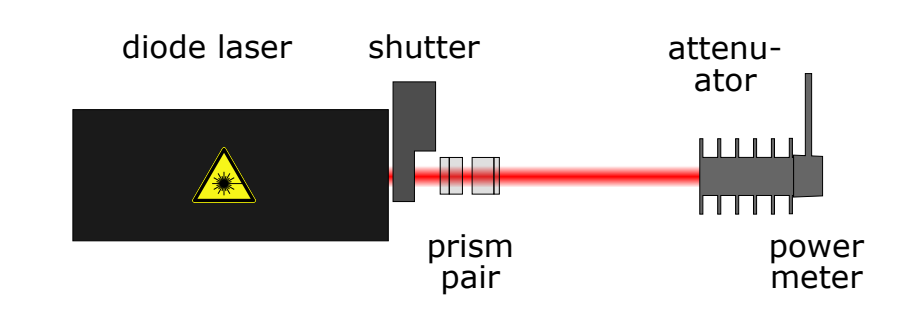
\includegraphics[scale=0.4]{./imagesandplots/pic1.png}
\centering
\caption{Set up to measure variation of laser output power with injection current \cite{UB}}
\label{figexpt1}
\end{figure}

The set up for this experiment (along with attenuator attached) is shown in Figure \ref{figexpt1}. With this setup in place, the injection current was increased from 0 to 280 mA in increments of 5 mA, and the corresponding values of output power were noted. Since the power meter sensor becomes non-linear for powers above 20 mW, it becomes necessary to use an attenuator. For our measurements, we took measurements both with, and without attenuator in the unattenuated power range from 28.2 $\mu$W to 19000 $\mu$W (19 mW). Both the unattenuated and attenuated power values are essential to be recorded over at least some data points in order to perform the calibration and extract a calibration factor from it. Beyond this range, the power was only measured with the attenuator attached onto the power meter, due to the aforementioned reason of non-linearity of the sensor. The attenuator for the experiment was a `1000:1' attenuator (meaning that ideally it reduces the unattenuated power by a factor of 1000). The recorded data can be found in \ref{tab1}. The values measured without attenuator are listed under the column `$P_{unatt}$' and the measured power values with attenuator are under the column `$P_{att}$'. From now on, all errors stated in the tables should be assumed to be instrumental errors (least count of the measuring instrument), unless otherwise stated.

\subsection{Calibration of removable attenuator}
\label{Calib}
In order to find the calibration factor, the data for the attenuated power vs. unattenuated power is plotted and a linear fit is applied to this dataset. To carry out the curve fitting procedure using the data points and some initial guess parameters, we used the function \texttt{curve\_fit()} from the \texttt{scipy.optimize} module for \textit{Python}. The data points (along with x-y error bars) and the linear fit modelled onto them is shown in Figure \ref{figexpt2}.

\begin{figure}[H]
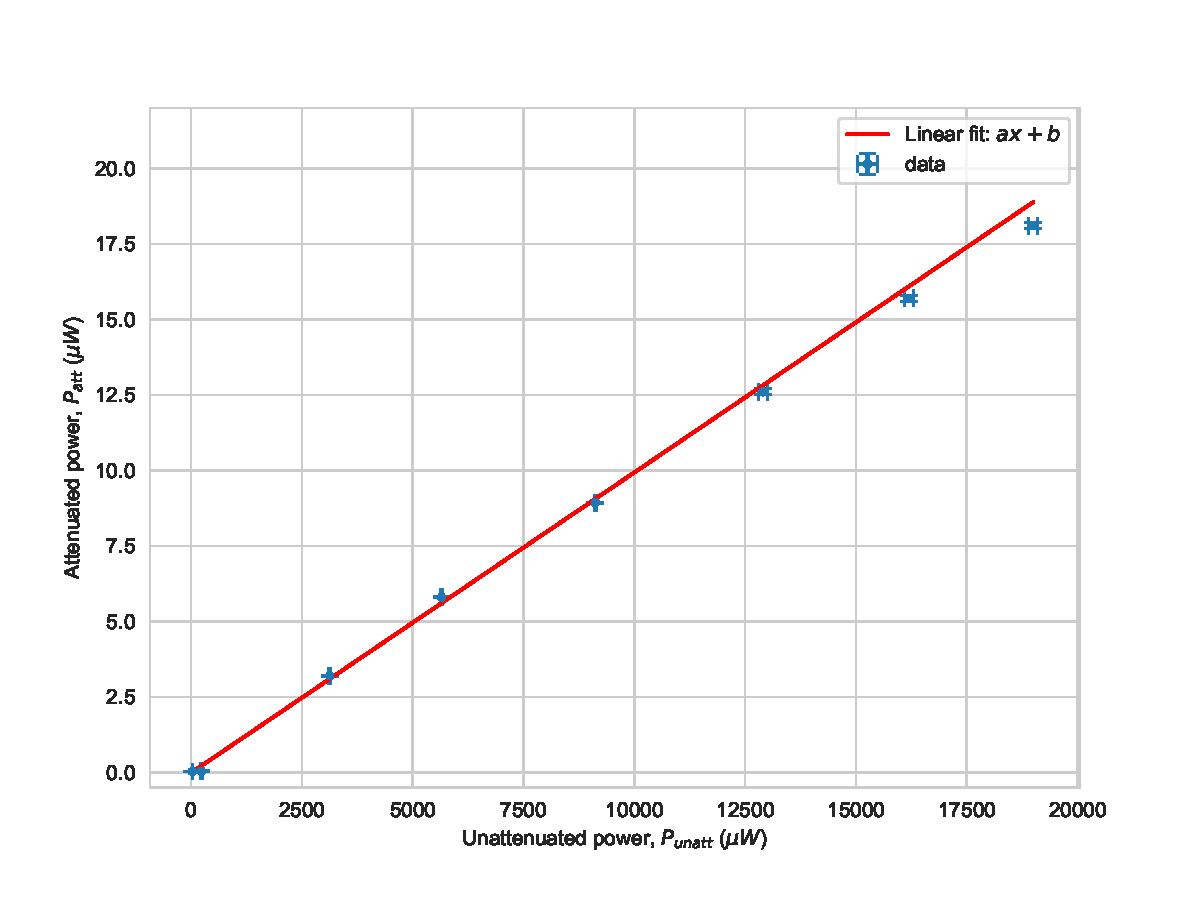
\includegraphics[width=0.9\textwidth]{./imagesandplots/attvsunattcalib.pdf}
\centering
\caption{Calibration plot of attenuated output power vs unattenuated power}
\label{figexpt2}
\end{figure}

The linear fit chosen is of the form: 
\begin{equation}
\label{eqn:linearfit1}
P_{att}=aP_{unatt}+b
\end{equation}

The choice of the initial guess parameters is taken as $a=0.001$ (since as already mentioned before, attenuated power is around 1/1000 of the unattenuated power, due to use of `1000:1' attenuator) and $b=0$ (y intercept expected to be a very small value, by visually extrapolating the data points). Indeed, after running the curve fitting procedure, we get fit parameters close to our initial guess: $a=0.000994\pm 1.25\times 10^{-6}$ and $b=-0.016\pm 0.006$, giving: $$P_{att}=(0.000994\pm 1.25\times 10^{-6})P_{unatt}+(-0.016\pm 0.006)$$
Now we use the commonly applied reduced $\chi^{2}$ test, to find the goodness of fit for this linear model: 
\begin{equation}
\chi^{2}=\sum_{i}\left[\dfrac{y_{i}(x_{i})-f_{i}(x_{i};p)}{\sigma_{i}}\right]^{2}
\end{equation}
where $y_{i}(x_{i})$ are the recorded y values (attenuated power in this case), $f_{i}(x_{i};p)$ is are y values from the fitting function with $p$ parameters (in this case the linear fit function with parameters $a$ and $b$).

Surprisingly, we get an extremely large reduced $\chi^{2}$ value of 174.69. Naively, one would conclude that since $\chi^{2}\gg 1$, the model is a `bad fit'. However, on looking more carefully at the data points, we make two observations:
\begin{itemize}
\item We find that the error in the first five data points (corresponding to current ($I$) values lying in the range of 50 to 70 mA) is an order of magnitude smaller than for the remaining data points. Given that the order $\mathcal{O}(y_{i}(x_{i})-f_{i}(x_{i};p))$ remains the same (more or less), the $\chi^{2}$ is sensitive to the order of the squares of the y-errors $\mathcal{O}(\chi^{2})\sim \mathcal{O}\left(1/\sigma_{i}^{2}\right)$. As such, the contribution from the very small errors of the first five data values would be around 100 times compared to that from the remaining y values.
\item Moreover, we only have a small number of data points ($N=8$), which we are trying to fit with two parameters ($p=2$), this restricts the degrees of freedom to only 6 ($df=N-p$). Again this leads to a large reduced $\chi^{2}$ value.
\end{itemize}
The combination of both these factors shows that in the case of small data sets, the error on the data points largely affects the reduced $\chi^{2}$ value. Indeed, this is confirmed in a paper by Andrae et.al. \cite{https://doi.org/10.48550/arxiv.1012.3754}. However, here, since we are concerned with only extracting the calibration factor, we just want to check how well the linear regression line approximates the actual data values. For this we calculate the $R^{2}$ (coefficient of determination): 
\begin{equation}
R^{2}=1-\displaystyle\dfrac{\sum_{i}\left(y_{i}-f_{i}(x_{i};p)\right)^{2}}{\sum_{i}\left(y_{i}-\bar{y}\right)^{2}}
\end{equation}
where $\bar{y}$ is the mean of all the recorded data values

The $R^{2}$ value indeed comes out to be very close to 1 ($R^{2}=0.997$), meaning that our linear model explains 99.7\% of all the variation of the y value (attenuated power) around its mean.

\subsection{Calculation of unattenuated power values above 19 $\mathbf{\mu}$W}
We recall that after the unattenuated power reached a value of 19 $\mu$W, only attenuated power values were recorded. Therefore, in order to find the dependence of unattenuated power with the injection current, we need to use to calculate unattenuated power values above 19 $\mu$W first, by applying the calibration factor to the attenuated power values. From Eq. \ref{eqn:linearfit1} we get:
\begin{equation}
\label{eqn:punattfrompatt}
P_{unatt}=\dfrac{P_{att}-b}{a}
\end{equation}
In addition to this, the errors on each of these calculated values will no longer be instrumental, but will be calculated from error propagation:
\begin{equation}
\label{eqn:errorprop1}
\Delta P_{unatt}=\sqrt{\left(\dfrac{\Delta P_{att}}{a}\right)^{2}+\left(\dfrac{\Delta b}{a}\right)^{2}+\left(\dfrac{\Delta a(P_{att}-b)}{a^{2}}\right)^{2}}
\end{equation}
These calculated unattenuated power values and their errors are also included in Table \ref{tab1}.

\subsection{Study of dependence of fundamental output power on the injection current}
Once all the unattenuated power values are obtained, the fundamental unattenuated power vs injection current is plotted. This plot is shown in Figure \ref{figexpt3}. 

\begin{figure}[H]
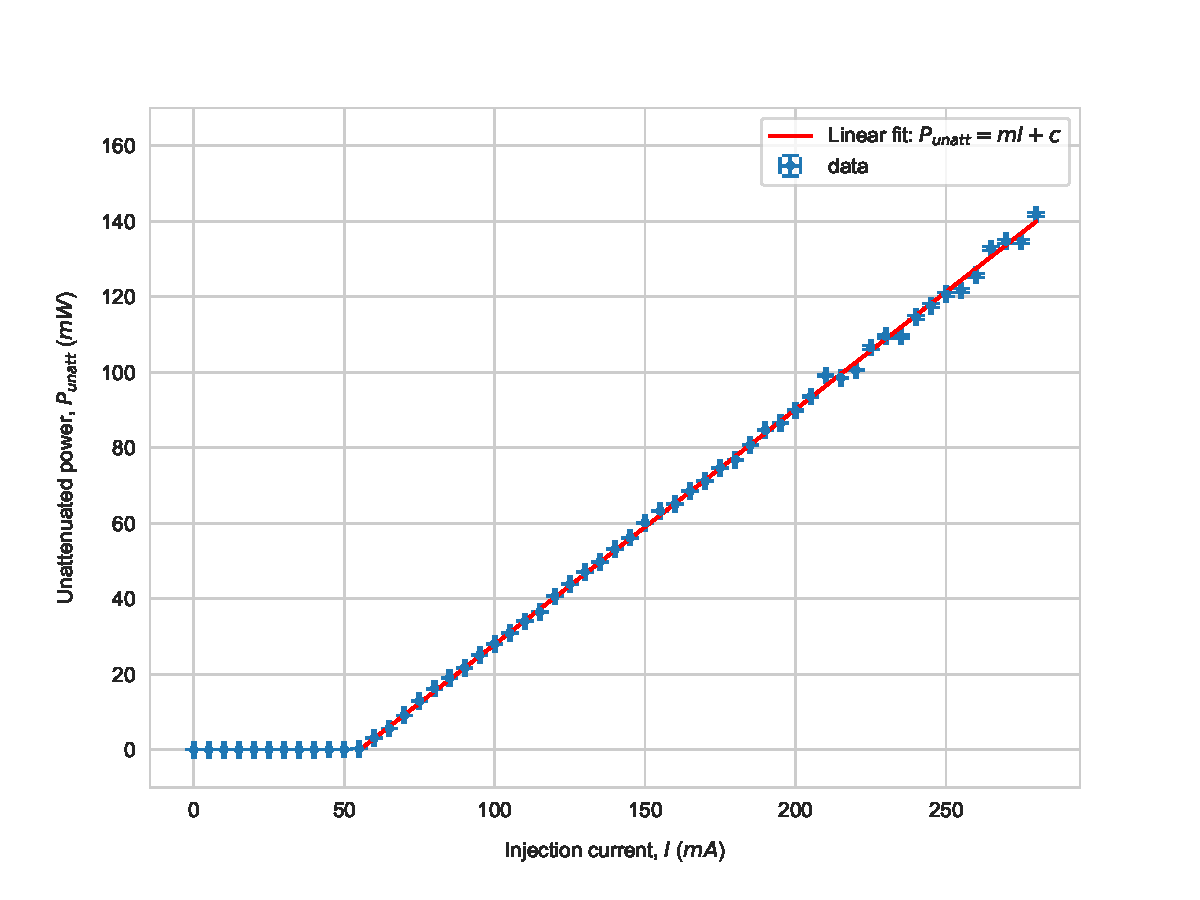
\includegraphics[width=0.9\textwidth]{./imagesandplots/injcvsunattpow.pdf}
\centering
\caption{Plot of unattenuated output power vs injection current}
\label{figexpt3}
\end{figure}

One finds that the unattenuated power remains close to zero upto a certain value of the injection current (around 50 mA) and after this value, the fundamental power starts increasing linearly with the injection current. As such, for this linear region, we choose a linear fit of the form: 
\begin{equation}
P_{unatt}=mI+c
\end{equation}  
After visually guessing the slope and the y intercept, we take initial parameters for curve fitting as $m=30/40=0.75$ and $c=-30$. The least square curve fitting procedure gives the best linear fit as: 
\begin{equation}
P_{unatt}=(0.62234\pm 0.00027)I+(-34.329\pm 0.022)\ \rm{mW}
\end{equation}
The $R^{2}$ value for this fit is found to be 0.9993, indicating a linear model that explains the variability in y values quite well. Again, the $\chi^{2}$ goodness of fit test isn't used here because of the complications mentioned in Section \ref{Calib}.

\subsection{Calculation of laser output characteristics}
\begin{itemize}
\item \textbf{Threshold current:} The particular value of injection current, at which the output unattenuated power starts increasing from zero is called the threshold current and is given by:
\begin{equation}
I_{0}=-\dfrac{c}{m}
\end{equation} 
while its error is found to be:
\begin{equation}
\Delta I_{0}=\sqrt{\left(\dfrac{\Delta c}{m}\right)^{2}+\left(\dfrac{c \Delta m}{m}\right)^{2}}
\end{equation}
This gives a threshold current value of $I_{0}=55.161\pm 0.039$ mA
\item \textbf{Differential slope efficiency:} The differential slope efficiency, in the case of this linear fit is simply the slope of the straight line:
\begin{equation}
\dfrac{\partial P}{\partial I}=\dfrac{P}{I}=m
\end{equation}
with its error given as:
\begin{equation}
\Delta \left(\dfrac{\partial P}{\partial I}\right)=\Delta m
\end{equation}
The result is then $\dfrac{\partial P}{\partial I}=-34.329\pm 0.022$ W/A
\item \textbf{Quantum efficiency:} The quantum efficiency is given by the ratio of the number of photons that are emitted ($N_{\gamma}$) to the number of injected electrons ($N_{e}$). This is then given as:
\begin{equation}
\eta=\dfrac{N_{\gamma}}{N_{e}}=\dfrac{e}{h \nu}\dfrac{\partial P}{\partial I}
\end{equation}
with error:
\begin{equation}
\Delta \eta=\dfrac{N_{\gamma}}{N_{e}}=\left(\dfrac{e}{h \nu}\right)\Delta\left(\dfrac{\partial P}{\partial I}\right)=\left(\dfrac{e\lambda}{hc}\right)\Delta\left(\dfrac{\partial P}{\partial I}\right)
\end{equation}
where $e$ is the fundamental unit of electric charge, $h$ is Planck's constant and $\nu$ is the frequency of light given as $c/\lambda$. The quantum efficiency is then found to be $\eta=0.495\pm 0.00021$. The interpretation of this value is that on an average, for every 2 ($\sim 1/\eta$) electrons injected into the laser diode, 1 photon was emitted.
\end{itemize}

\subsection{Calibration of variable attenuator}
We observed that controlling the laser fundamental power by varying the diode current is an inefficient method since the power of the laser did not vary continuously with the injection current. Instead jumps in power and frequency occurred when we did this (known as `mode hops') \cite{UB}. Therefore the previous setup was modified by introducing a rotatable $\lambda /2$ plate and a beam splitter cube (both of which function as two polarizers), in the beam path between the laser diode and the power meter. The injection current was fixed at its maximum value for this part of the experiment. First, we checked that the beam splitter cube was placed such that it transmitted the maximum possible power without the $\lambda /2$ plate. After this was ensured, the $\lambda /2$ plate was inserted. Moreover, as done before, in order to precisely adjust the heights and positions of the optical elements, an IR card was used to follow the beam path and ensure that the entire transmitted beam falls completely on the power meter. The schematic set up for this part of the experiment is shown in Figure \ref{figexpt4}.

\begin{figure}[H]
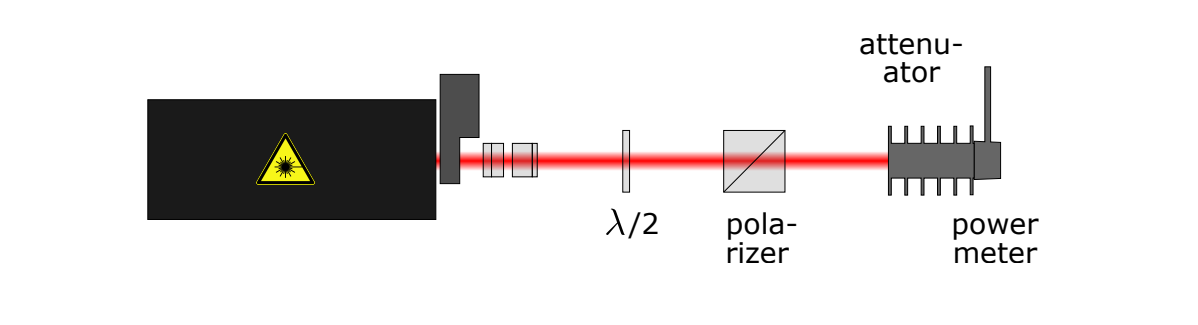
\includegraphics[scale=0.4]{./imagesandplots/pic2.png}
\centering
\caption{Schematic set up for variable attenuator calibration \cite{UB}}
\label{figexpt4}
\end{figure}

Now, in order to find the dependence of transmitted fundamental power with the angle of polarization, we rotated the $\lambda/2$ plate in a clockwise direction, starting from $0\degree$ upto $180\degree$ in increments of $2.5\degree$. A non linear, $\cos^{2}\theta$ form of fitting curve is chosen for this data, since we expect this variation to follow Malus' law. Both the plot of this variation along with the fitting curve are displayed in Figure \ref{figexpt5}.

\begin{figure}[H]
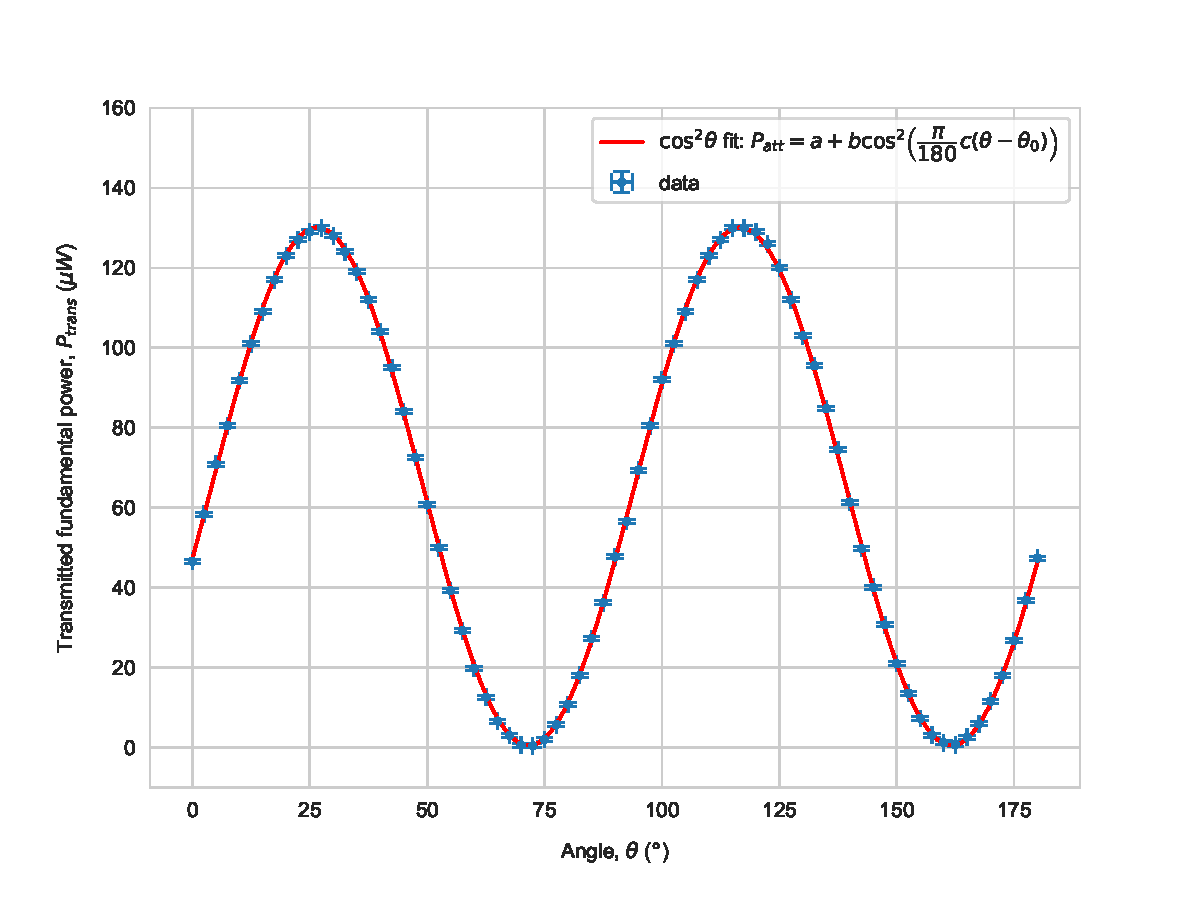
\includegraphics[width=0.9\textwidth]{./imagesandplots/variabattcalib.pdf}
\centering
\caption{Plot of the transmitted fundamental power vs the rotation angle of the $\lambda /2$ plate}
\label{figexpt5}
\end{figure}

The exact form of the fitting function is taken as follows:
\begin{equation}
P_{trans}=a+b\cos^{2}\left(\dfrac{\pi}{180}c(\theta-\theta_{0})\right)
\end{equation}
where the parameter $a$ represents the minimum transmitted power, $b$ represents the difference between the maximum and minimum transmitted power, $c$ being the factor by which the beam was rotated by the $\lambda /2$ plate and $\theta_{0}$ representing the angle of $\lambda /2$ plate at which maximum power was measured. The factor of $\pi / 180$ is simply there to convert the measured angles in degrees to radians since the cosine function, \texttt{numpy.cos()} used in \textit{Python} accepts angles in radians. By visually inspecting the plots of the data points, the initial guess parameters for the fitting function are taken as: $a=0$, $b=130$, $c=2$ (expected to be 2 since a rotation of the $\lambda /2$ plate by $\theta$ would rotate plane of polarization of the initial beam by 2$\theta$), $\theta_{0}=0$. After fitting, the optimal parameters come out to be:
\begin{align*}
a&=(0.540\pm 0.102)\ \mu\rm{W}\\
b&=(129.561\pm 0.167)\ \mu\rm{W}\\
c&=1.9983\pm 0.0007\\
\theta_{0}&=(26.590\pm 0.027)\degree
\end{align*}

As the data in this case is free from the complications discussed in Section \ref{Calib}, we use the $\chi^{2}$ test for goodness of fit. The reduced $\chi^{2}$ value comes out to be 1.47, which tells us that that the model $\cos^{2}\theta$ curve fits the data well enough. 

Given that we now have a calibration curve that describes the variation of transmitted fundamental power with the polarization angle, it is possible to measure just the variation of second harmonic power with the angle, $\theta$ to in turn get the dependence of second harmonic power on fundamental power, using the calibration curve. \label{variablecalib}

Additionally, we calculate the extinction ratio, which is defined as the ratio of the maximum transmitted power to minimum transmitted power:
\begin{equation}
\eta_{ext}=\dfrac{P_{max}}{P_{min}}=\dfrac{a+b}{a}
\end{equation}
with its error as:
\begin{equation}
\Delta \eta_{ext}=\sqrt{\left(\dfrac{\Delta b}{a}\right)^{2}+\left(\dfrac{b\Delta a}{a^{2}}\right)^{2}}
\end{equation}
This gives us an extinction ratio of $\eta_{ext}=240.683\pm 45.024$

\section{Second harmonic wave generation}
In this part of the experiment, the laser beam is directed into the non-linear crystal ($\rm{KbNO_{3}}$, potassium niobate) and variations of the second harmonic power with different parameters (such as the crystal temperature, fundamental wave power and angle of polarization of fundamental wave) is recorded.

\subsection{Focusing the laser beam into the non-linear crystal}
The first step for second harmonic wave generation was to devise a method to focus the laser beam into the crystal and subsequently collimate the light transmitted through the crystal. The diagram of the entire set up is displayed in Figure \ref{figexpt6}

\begin{figure}[H]
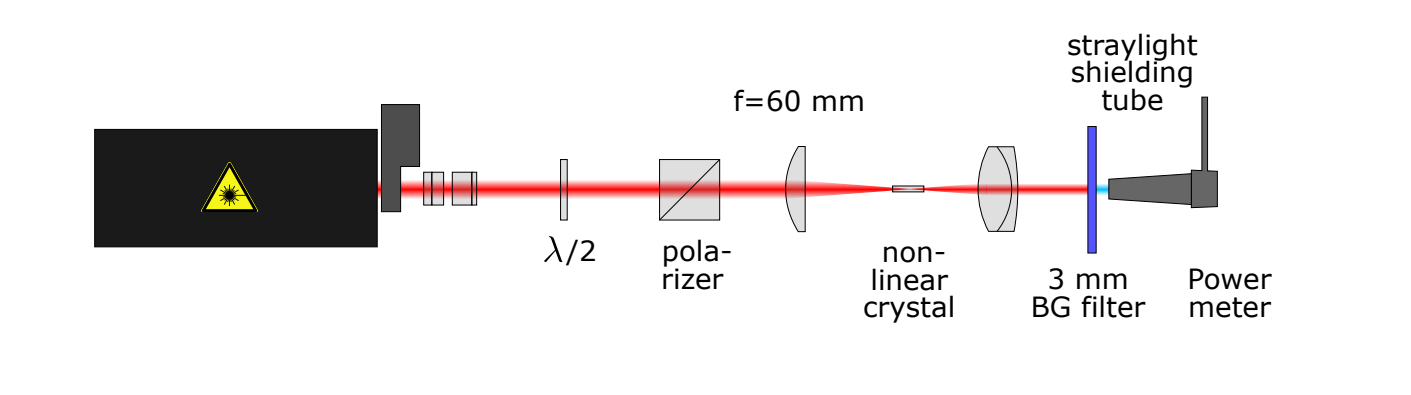
\includegraphics[scale=0.4]{./imagesandplots/pic3.png}
\centering
\caption{Arrangement for focusing of fundamental wave and subsequent collimation of light transmitted through the non-linear crystal \cite{UB}}
\label{figexpt6}
\end{figure}

The focusing lens was necessary to ensure that the entire intensity of the incident beam entered the non-linear crystal, which would then mean that a second harmonic beam having the maximum possible power/intensity would be generated. In order to accomplish this, we used a plano-convex lens with a focal length of $f=$60 mm. The lens was placed such that its convex surface faced the incoming beam and the plane surface faced the opposite direction. We noted that in order for the incident beam to be maximally focused when it enters the crystal, the distance between the focusing lens and the crystal needs to a  equal to the focal length (60 mm) of the lens. This distance was measured with a scale and the position where the lens would then be placed is marked. However, before placing the lens, we needed to ensure that the beam fell exactly on the center of the focusing lens. To do this, we used a screen (which in this case was an upright stand with paper taped onto it) and placed it at some distance further from where the lens was to be placed. With the help of an IR card, the size of the laser beam spot was marked on the screen. Now, the focusing lens was placed at the decided position and finer adjustment of its position was done so that the beam falling on the screen now had a spot that exactly overlapped the one marked before placing it. Another consideration was that the lens surface had to perpendicular to the beam path, i.e the optical axis of the lens needed to be aligned with the beam path. This was important because deviation of the optic axis from the beam path would produce undesirable effects such as coma and astigmatism \cite{UB}. To do this we first checked if the beam path was itself parallel to the surface of the optical table as well as to the rows of holes on it. Then, it was visually ensured that the lens surface was perpendicular to the table and to the incoming beam axis. The rows of holes on table again assisted us in doing this. Finally, the lens was clamped at the optimal position.   

Now, the fundamental beam was transmitted through the crystal and using the IR card, it could be seen on the other side. However, this beam was slightly diverging and in order to get the maximum power measurement at the power meter, we needed to use a collimating lens. The lens used for this purpose was again a plano-convex lens (having a focal length of 30 mm), with its convex surface now facing the incoming beam. As done before, this lens was placed at distance equal to its focal length, away from the crystal. Again, it was visually ensured that the lens was upright (perpendicular to the table) and also perpendicular to the beam path. Finer adjustment of the lens position (along beam axis) was made by moving the screen over an appreciable distance along the (supposedly) collimated beam path and observing if the beam spot size remains the same (with the help of the IR card). After all these adjustments, the collimating lens position was finalized and it was clamped to the optical table.

\subsection{Optimizing the second harmonic power}
In order for us to clearly observe the second harmonic wave generated by the crystal, we needed to bring the crystal to a temperature where it gives maximum intensity of second harmonic light. For the case of the $\rm{KbNO_{3}}$ crystal, it is found to be around 36.7 $\degree$C \cite{UB}. Therefore, in the present experiment, the crystal was slowly heated up from 27 $\degree$C to 36.7 $\degree$C in small increments of 0.5 $\degree$C. Once this peak temperature was reached, with the crystal properly aligned with the beam direction, we could clearly see a blue light spot on the screen placed after the lens (along the direction of beam propagation), indicating that the SH (second harmonic) light had been generated. 

The crystal arrangement had been mounted onto a stand that had threaded screws for finer adjustment of crystal position in all three directions. In order to perfectly optimize the intensity of SH light generated, the power meter was turned on, its wavelength setting was set to 493.5 nm (half of the fundamental wavelength) and the power reading was noted. Using the threaded screws on the aforementioned arrangement, the crystal position was fine tuned, so that a maximum value of power was measured. While fine tuning, it was noticed that the SH power goes down significantly if the fundamental beam falls on to the edges to the crystal (since it will then not be entirely converted to SH light), therefore crystal position was adjusted so that the beam was incident at the center of the crystal. The generation of the SH blue light illuminated the crystal edges clearly, which made it easy for us to do this adjustment. Since only the SH power was to be recorded, a BG40 glass filter, of thickness 3 mm was used to block out the infrared fundamental wave component. Further, in order to prevent any background signal from affecting the actual SH reading, we mounted a conical stray-light shielding tube onto the measuring surface of the power meter. All readings that would be subsequently be reported in this section, had been recorded with the stray-light shielding tube attached. 

On optimization, the SH beam power was found to have a maximum value of 36.6 $\mu$W which is slightly lower than the desirable optimal value of 40 $\mu$W \cite{UB}. This can be attributed to the fact that the theoretical value of 36.7 $\degree$C might not exactly be the temperature at which the SH intensity is maximum. This temperature was later on adjusted more precisely while studying dependence of SH power on crystal temperature.

\subsection{Calculation of Gaussian beam parameters}
The next step would be to check how close the parameters of the generated SH beam are to the optimal values of Gaussian beam parameters. To this end, we first list out some pre-calculated parameters and constants given in lab instruction manual \cite{UB}. (Note: values of focal length, refractive index, length of crystal and wavelength have been stated without any associated errors in the manual, and therefore they have been taken as such). 
\begin{itemize}
\item Crystal refractive index, $n=2.2$
\item Fundamental beam wavelength, $\lambda=987$ nm
\item Focal length of focusing lens, $f=60$ mm
\item Length of non-linear crystal, $L=5$ mm
\item Beam diameter before entering lens, $d=(3.5\pm 0.5)$ mm 
\end{itemize}

Now, we calculate the beam parameters:
\begin{itemize}
\item \textbf{Beam waist:} The beam waist is given by: 
\begin{equation}
\omega_{0}=\dfrac{2f\lambda}{\pi d}
\end{equation}
and its error is calculated as:
\begin{equation}
\Delta \omega_{0}=\dfrac{2f\lambda}{\pi}\left(\dfrac{\Delta d}{d}\right)
\end{equation}
This gives us a value of $\omega_{0}=10.771\pm 5.386$ $\mu$m
\item \textbf{Rayleigh length:} The Rayleigh length is defined as:
\begin{equation}
z_{0}=\dfrac{\pi n \omega_{0}^{2}}{\lambda}
\end{equation}
and has an error:
\begin{equation}
\Delta z_{0}=\dfrac{2\pi n \omega_{0}\Delta \omega_{0}}{\lambda}
\end{equation}
We get the value of Rayleigh length as $z_{0}=0.812\pm 0.406$ mm
\item \textbf{Confocal parameter:} The confocal parameter is given as:
\begin{equation}
b=2z_{0}
\end{equation}
with an error:
\begin{equation}
\Delta b=2\Delta z_{0}
\end{equation}
This gives a value of $b=1.625\pm 0.812$ mm
\item \textbf{Boyd Kleinman condition:} For maximal efficiency of SH wave power generation, one needs to have the crystal length ($L$) and confocal parameter ($b$) in the ratio: 
\begin{equation}
\dfrac{L}{b}=2.84
\end{equation}
with the error calculated as: 
\begin{equation}
\Delta \left(\dfrac{L}{b}\right)=\dfrac{L\Delta b}{b^{2}}
\end{equation}
Putting in the values of $L$ and $b$ in our case, we get the ratio as: $L/b=3.077\pm 1.538$. We see that this value for our set up is close to the optimal value, within the calculated error bounds.
\item \textbf{Optimal focal length:} The optimal focal length for this experiment can be calculated by using the obtained Boyd-Kleinman ratio and substituting the expression for $b$ in terms of focal length ($f$), and then solving the equation:
$$
\dfrac{L}{b}=\dfrac{L}{2z_{0}}=\dfrac{\lambda L}{2\pi n \omega_{0}^{2}}=\dfrac{\pi d^{2} L}{8nf^{2}\lambda}=3.077
$$
This gives us: 
\begin{equation}
f_{opt}=\sqrt{\dfrac{\pi d^{2}L}{24.616n\lambda}}
\end{equation}
with an error: 
\begin{equation}
\Delta f_{opt}=\sqrt{\dfrac{\pi L}{24.616n\lambda}}\Delta d
\end{equation}
The value obtained for the optimal focal length is then $f_{opt}=60.000\pm 8.571$ mm. Clearly this matches with the focal length of the lens that we have used, although we find that there is a large theoretical uncertainty on it as calculated from the error propagation.
\end{itemize}

\section{Dependence of second harmonic wave power on different variables}
For this part of the experiment, the properties of the SH beam power had to be studied by finding its relation to the crystal temperature, fundamental wave power and the fundamental wave polarization. It is to be noted that although the manual instructs us to first study the variation of the SH power to crystal temperature, we performed this part at the end, since given that the crystal was already heated up to (nearly) its optimal temperature, it was feasible to readily record SH power variation with fundamental beam power and polarization, without disturbing the temperature of the crystal. 

\subsection{Variation of harmonic power with fundamental wave power} 
For studying this dependence, we find that the power meter cannot be moved each time to measure both the power of the fundamental power as well as SH power. Therefore, as discussed towards the end of Section \ref{variablecalib}, we measured the dependence of the SH power on the rotation angle of the $\lambda /2$ plate and used the calibration curve obtained to find the direct dependence between SH beam power and the fundamental beam power. In addition to this, it is to be noted that while we measured the SH power without attenuator in this experiment, the fundamental power was measured with the attenuator attached to the power meter, while doing the calibration in Section \ref{variablecalib}. The recorded values are given in Table \ref{tab:shpowvsfundpow}.

\label{anomaly}
It is to be noted that while these readings were being taken by varying the rotation angle of the $\lambda /2$ plate, a drastic drop in SH power was observed after an angle of $122.5 \degree$. While the SH power was found to be 32.6 $\mu$W at $122.5 \degree$, it decreased significantly to 22.2 $\mu$W at $125 \degree$, and then kept decreasing gradually below this value as rotation angle was increased. When the $\lambda /2$ plate was rotated back to the angle ($27.5 \degree$) at which SH power had earlier attained a maximum of 36.6 $\mu$W ; we now recorded only a peak value of 25.4 $\mu$W. In order to get back the former value of SH power, attempts were made to fine tune the position of the crystal in all three directions, however it was not possible to recover from this drop of about 11.2 $\mu$W. The only reasons that this drop in SH power could have happened are that there might have been a sudden temperature fluctuation of the laser itself or that that the wavelength emitted by the laser diode changed slightly, again due to some internal instability. Given that it was not possible to account for these changes, we continued our observations with this new reduced value of SH power. The plot of the variation of the SH power (unattenuated) with fundamental power (attenuated) only upto the aforementioned angle of $122.5 \degree$ is displayed in Figure \ref{figexpt7}.

\begin{figure}[H]
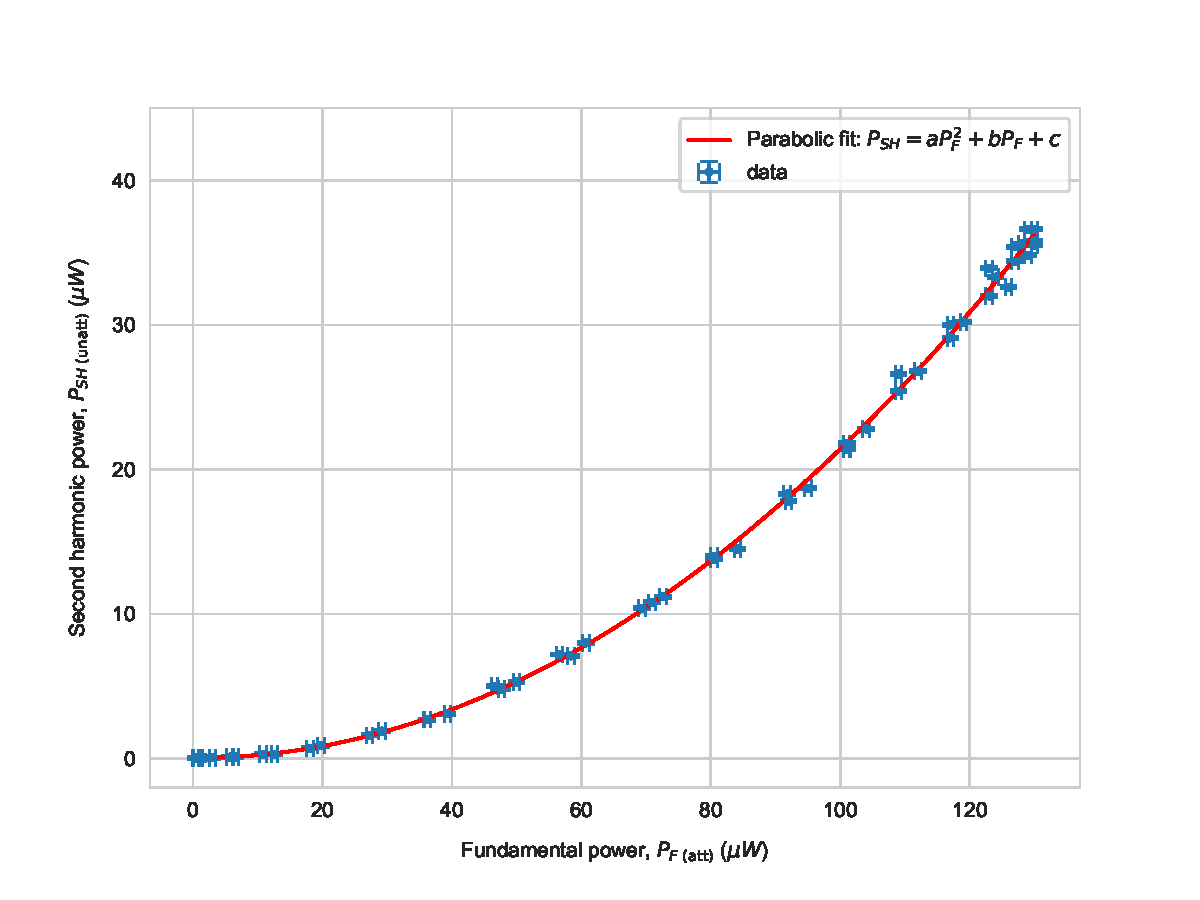
\includegraphics[width=0.9\textwidth]{./imagesandplots/shpowvsfundpow.pdf}
\centering
\caption{Plot of the second harmonic (unattenuated) power vs the fundamental (attenuated) power}
\label{figexpt7}
\end{figure}

From the theory \cite{yarivqm}, we expect the SH power to depend on the fundamental power as: 
\begin{equation}
P_{SH}=\eta P_{F}^{2}
\end{equation}
where $\eta$ is the efficiency.
Thereforem to fit this curve, we choose a model following general form of a parabola:
\begin{equation}
P_{SH}=aP_{F}^{2}+bP_{F}+c
\end{equation}
We take initial guess parameters as: $a=1/500$ (we used this because, $x$ value of 100 gives a $y$ value of around 20; assuming quadratic dependence, this would give the factor to be multiplied with $x^{2}$ as $20/10000=1/500$), $b=0$ (linear dependence is assumed to be very small) and $c=0$ (no offset can be seen from the $x$-axis). The curve fitting module yields the following optimal parameter values:
\begin{align*}
a&=(0.0022\pm 9.3988\times 10^{-6})\ \mu\rm{W}^{-1}\\
b&=-0.0031\pm 0.0013\\
c&=(0.0562\pm 0.0367)\ \mu\rm{W}
\end{align*}  
We find that while $a$ has a very small error relative to its calculated value, the errors in parameters $b$ and $c$ are of the same order of magnitude as the values themselves. Since these two parameters can be affected heavily by their own statistical errors, they can be regarded as unimportant and we can say that the data points approximately follow the relation $P_{SH}\approx\eta P_{F}^{2}$. The efficiency $\eta$ is same as the optimal value of parameter $a$ and is therefore: 
\begin{equation}
\eta=(0.0022\pm 9.3988\times 10^{-6})\ \mu\rm{W}^{-1}
\end{equation}

Although it can be clearly seen that the data points follow this parabolic variation well, the reduced $\chi^{2}$ value comes out to quite large ($\chi_{red}^{2}=24.42$). This could be due to the fact that while the data points lie (more or less) on the fit curve at lower values of fundamental power; at higher values (from above 100 $\mu$W) some of the data points are scattered a little away from the fit curve. Since the errors on each of the data points are already small, this contributes to a large $\chi_{red}^{2}$ value. Moreover, as discussed in the paper by Andrae et.al. \cite{https://doi.org/10.48550/arxiv.1012.3754}, the $\chi^{2}$ test should not always be used as a test of goodness of fit, since for non-linear models, the degrees of freedom isn't always given by $df=N-p$ (where $N$ is the number of points and $p$ the number of fit parameters) and may not even be constant during the fitting procedure. 

\subsection{Variation of harmonic power with polarization of fundamental wave}
For this part of the experiment, we removed the beam splitting polarizer from the arrangement, so that the polarization of the fundamental wave could be changed by changing the rotation angle of the $\lambda/2$ plate. As done before, the angle of polarization was varied from $0 \degree$ to $180 \degree$ in increments of $2.5 \degree$. The recorded values can be found in Table \ref{tab:shpowvspol}. 

While Type I phase matching gives a dependence of $P_{SH}\propto \cos^{4}\theta$, Type II phase matching condition would give a $P_{SH}\propto \cos^{2}\theta\sin^{2}\theta$ dependence. In order to find which of these phase matching conditions holds true for our experiment, we design two non linear fits of the form:
\begin{align}
P_{SH}&=a\cos^{4}\left(\dfrac{\pi}{180}b(\theta-\theta_{0})\right)+c\\
P_{SH}&=a\cos^{2}\left(\dfrac{\pi}{180}b(\theta-\theta_{0})\right)\sin^{2}\left(\dfrac{\pi}{180}b(\theta-\theta_{0})\right)+c
\end{align}

\subsection{Variation of harmonic power with crystal temperature}
In order to to study the dependence of the SH power on the crystal temperature, we decided that it would be more feasible to first increase the temperature of the crystal upto a maximum possible 39.9 $\degree$C (in small steps of 0.2 $\degree$C), since the crystal was already set at a temperature of 36.7 $\degree$C; and then gradually decrease the temperature upto a minimum possible of 26.9 $\degree$C. It is also to be noted that while the readings were taken in steps of 0.2 $\degree$C down till 34.4 $\degree$C, while going further below this temperature, the reading of the power meter did not change much and therefore the steps were taken to be 0.5 $\degree$C in this range, in order to be time efficient. The recorded observations are given in Table \ref{tab:crysttemp}.
 

\section{Comparison of wavelengths of second harmonic and fundamental waves}
\subsection{Wavelength comparison using a diffraction grating}
 
In this part, we would like to calculate the wavelengths of the fundamental beam and the second harmonic using a setup involving diffraction grating, the principles of which were discussed earlier. The setup is shown in the figure \ref{fig:diffgrat}.
\begin{figure}
    \centering
    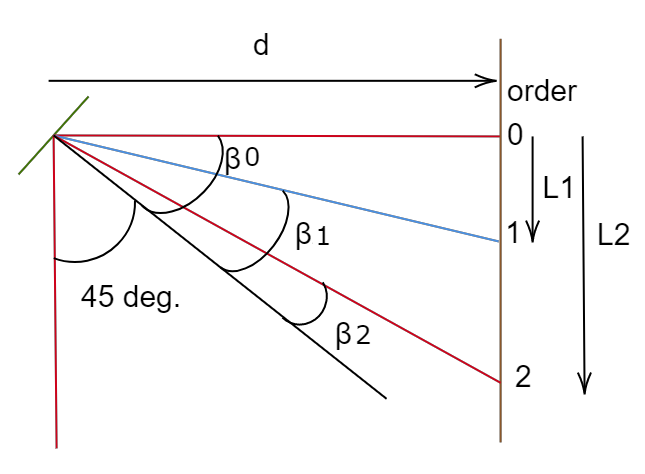
\includegraphics[width = 6cm]{diffgrat.png}
    \caption{Schematic of the setup to calculate the wavelengths using diffraction grating. The green line on top left corresponds to the diffraction grating, red lines correspond to beams of fundamental frequency and blue line correspond to beam of second harmonic frequency. The black line corresponds to the perpendicular to the grating.}
    \label{fig:diffgrat}
\end{figure}
The setup involved here is not sophisticated and we use regular measuring sticks to measure the distances. This comes with the drawback of having not a great error estimation. In our case, we assume a constant error of $0.5cm$ in all our readings, due to the scale of the measuring stick. We also achieve the angle of $45^{\circ}$ by approximately aligning the $0$ order diffraction to lie perpendicular to the incoming beam. We should note that this crude alignment could add to the errors in our calculations, which we have no way of estimating.\\
From the figure \ref{fig:diffgrat}, we can calculate the following quantities,
\begin{equation}
\begin{split}
    \theta_m &= tan^{-1}\left(\frac{L_m}{d}\right) \\
    \beta_m &= \frac{\pi}{4} - \theta_m \\
    s_m &= sin(\pi/4) - sin(\beta_m),
\end{split}
\end{equation}
where the quantity $\theta_m$, which is not labelled in the figure, corresponds to the angle made by the $m^{th}$ order diffraction beam with the $0^{th}$ order beam. Then the rest of the calculations follow, with $L_m$ as the distance of the $m^{th}$ maximum from the $0^{th}$, $d$ is the distance of the screen from the grating. Then the wavelength is calculated as,
\begin{equation}
    \lambda = \frac{s_m D}{m},
\end{equation}
where D is the grating constant $\frac{1}{600} mm$. The error is calculated as,
\begin{equation}
    \Delta\lambda = \frac{cos(\beta_m)\Delta\theta_m D}{m},
\end{equation}
where $\Delta\theta_m = \frac{1}{L^2 + d^2}\sqrt{(L\Delta d)^2 + (d \Delta L)^2}$. The calculated wavelength can be found in the table \ref{tab:diffgrat}.
\begin{table}[]
    \centering
    \begin{tabular}{c|cccc}
         & L [m] & $\lambda$[nm] & $A_{exp}$ & $A_{th}$ \\
        \hline
        SH: 1st order & 66 & 497.5 $\pm$ 4.1 & 121.1 & 1800 \\
        SH: 2nd order & 137.8 & 495.5 $\pm$ 4.9 & 264.7 & 3600 \\
        SH: 3rd order & 246.4 & 488.6 $\pm$ 0.9 & 537.6 & 5400 \\
        Fund.: 1st order & 137.8 & 991.0 $\pm$ 3.7 & 264.7 & 1800
    \end{tabular}
    \caption{Positions of the different order diffraction maxima and the corresponding calculated wavelength. The last two columns correspond to the experimental and theoretical resolution.}
    \label{tab:diffgrat}
\end{table}
Therefore, we calculate the wavelength of the fundamental beam as $\lambda_{Fun} = 991.0 \pm 3.7 nm$ and for the wavelength of the second harmonic, we perform a weighted mean on the calculated values with the weights being inverse variances, giving us $\lambda_{SH} = 490.2 \pm 1.6 nm$. The literature value for these two quantities are $987nm$ and $493.5nm$ respectively. We notice that the literature values lie within $2\sigma$ of the calculated values, which is impressive considering the very crude setup. We also, calculate the ratio of the wavelengths of the fundamental beam to that of the second harmonic, which gives us,
\begin{equation}
    \frac{\lambda_{Fun}}{\lambda_{SH}} = 2.021 \pm 0.008.
\end{equation}
The calculated ratio reflects the fact that the calculated wavelength of the fundamental beam is slightly above the literature value, whereas the calculated wavelength of the second harmonic is slightly below the literature value. The ratio from the literature values lie within $3\sigma$ of our ratio. We comment that we have not included all the possible errors in the setup and only take the major source of error which is the error in the measuring stick, which is also taken as a constant. The ignored errors add up to produce an unpredictable final error in our result. To achieve greater efficiency, a much more sophisticated setup is to be aimed for. We also have the experimental resolution, $A_{exp} = \frac{\lambda}{\Delta\lambda}$ and the theoretical resolution, $A_{th} = m \times N$ in the table \ref{tab:diffgrat}. In our case, $N$, which is the number of illuminated lines, was calculated approximately as $1800$, with the diffraction constant being $600$ lines/$mm$ and the beam width of the laser being $3mm$. Even though the experimental resolution is far from the theoretical resolution, we can observe the linear dependence on the order of magnitude $m$. We posit that the low experimental resolution values are due to the high uncertainties in the calculated wavelength. With our setup, we were unable to measure the positions of the maxima to a greater precision, even though the diffraction maxima were sharp.

\subsection{Wavelength comparison using a Michelson interferometer}

In order to carry out this measurement, the collimating lens of focal length $f=30$ mm, is put back in place of the second lens. This is done since its necessary to have a very collimated beam for the interferometer to work well and also alignment of the interferometer becomes easier. The complete setup of the interferometer can be seen in fig. 10. After the second lens a thin filter is installed to damp the power of the fundamental wave since the used photodiode would be saturated by the full primary power. Further down the optical axis a mirror has been installed. Its azimuthal angle was fixed by rotating it perpendicular to the beam line. In this position the incoming beam should be reflected exactly onto itself. By poking a hole into a piece of paper and holding it such that the primary beam surpasses it before the mirror the two beams can easily be adjusted. Now the mirror is rotated such that it deflects the beam by 90° onto the movable end mirror. Now this mirror can be adjusted using the
same trick with the piece of paper as before, but this time both angles have to be fine tuned. When this mirror is completely adjusted the beam-splitter can  be put into place along with the fixed end mirror. After that the beam-splitter is adjusted such that the deflection angle is 90 $\degree$. The fixed end mirror is adjusted similar to the other two mirrors. As the last step of the setup the alignment of all beams is checked at a greater distance and the photodiodes are installed.
Those have to be adjusted such that the beam hits them centrical. To separate the fundamental wave from the second harmonic the 3mm-filter is used since its transmission of the fundamental wave is nearly zero but the reflection is high enough to use it as a mirror. Now the two photodiodes can be connected to the oscilloscope which is operated
in XY -mode. By slightly bumping against the optical table one can see the change of Lissajous figures on the oscilloscope one of which is exemplary shown
in fig. 11. With this setup we can then determine the wavelength relation of the two waves. To do this the mirror is moved such that one of the Lissajous figures discussed in the theory is visible. This displacement is then set to represent zero phase shift. After moving the mirror such that another figure of defined phase shift can be observed the displacement is noted. This process is repeated for as many orders as possible. The obtained data can be found in tab. 7.